\section{Results}

\subsection{Data}

Sktiser index data på log scala + evt. tabel over aktivers perfomance over periode - thats it.


\subsection{In-sample training: Tuning hyperparameters}

\begin{itemize}
    \item Sample period
    \item method - what do we maximize
    \item go over each tuning parameter separately.
\end{itemize}

\textbf{Maximize portfolio Sharpe, excess return and minimize annual turnover over the hyperparameters}

\subsection{Out-of-sample results}

\begin{itemize}
    \item Plot allocations
    \item Plot portfolio performance
    \item Table summarizing KPIs
\end{itemize}

\begin{figure}[H]
    \centering
    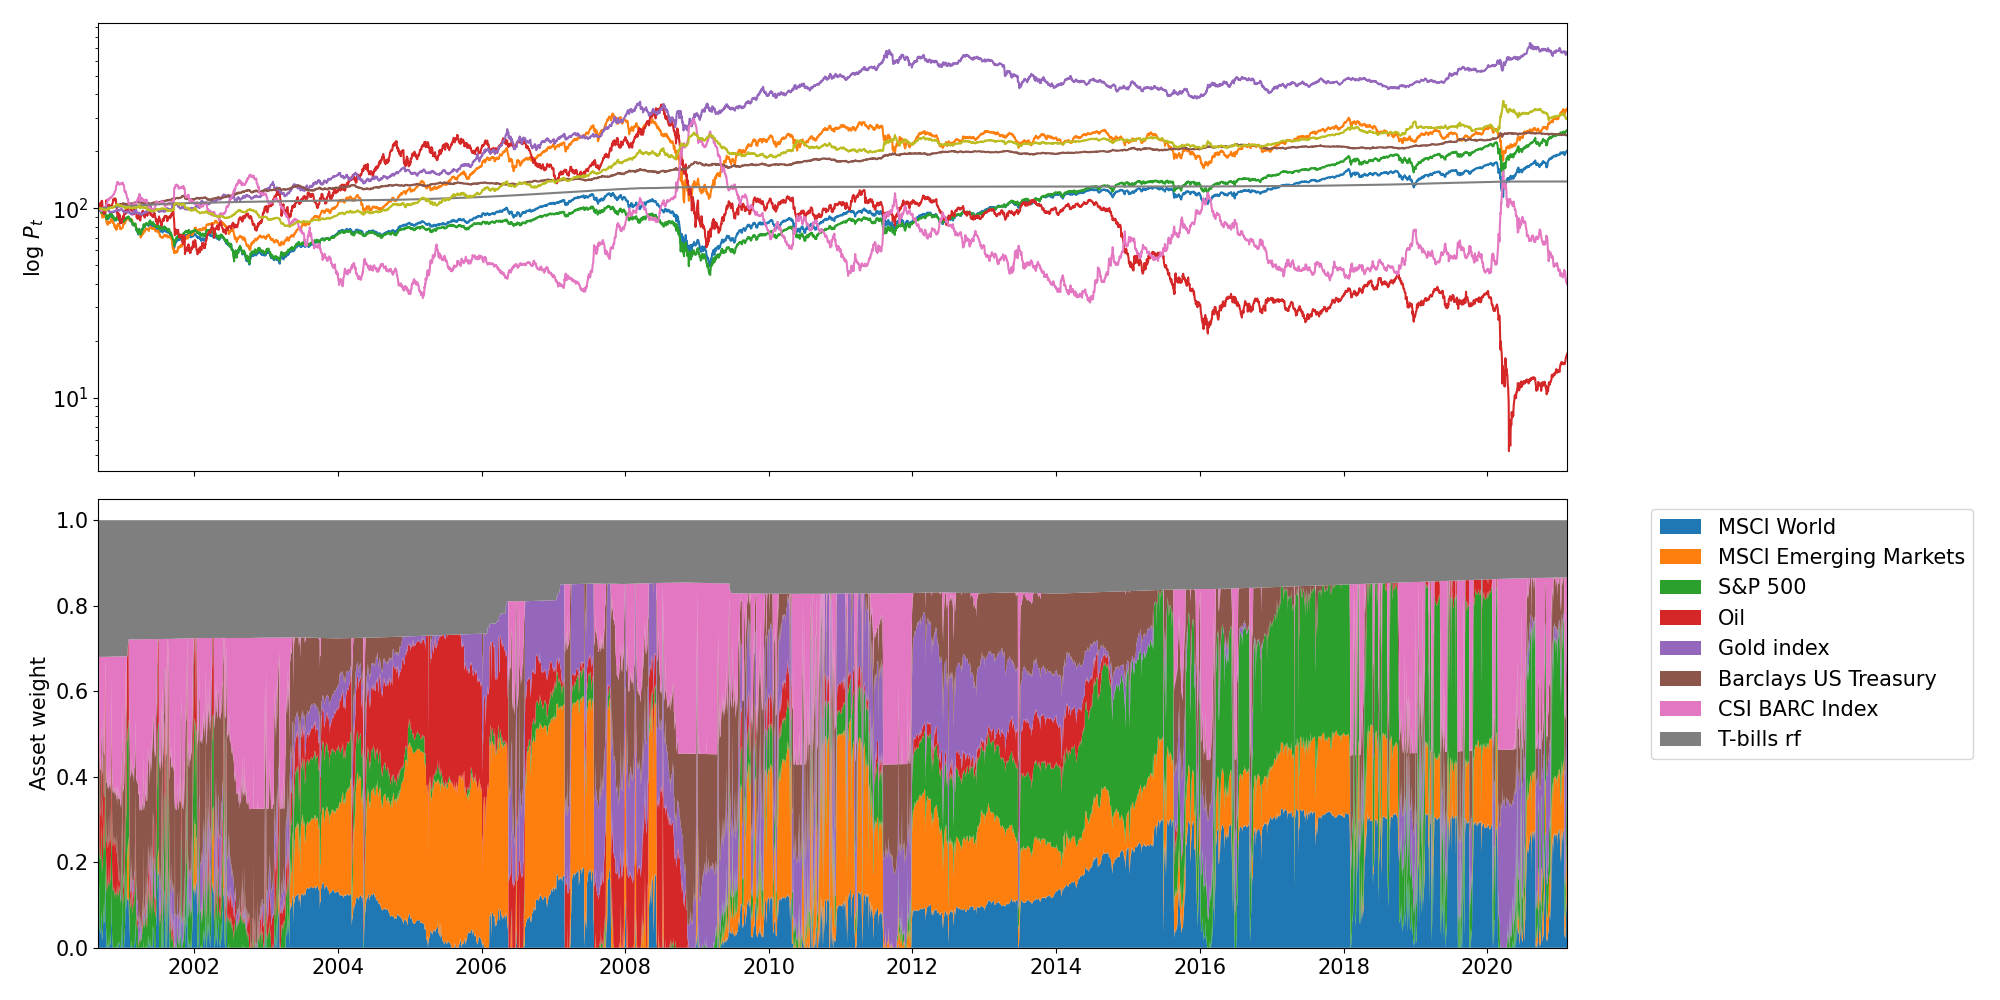
\includegraphics[width=1\textwidth]{analysis/portfolio_exercise/images/port_performance.png}
    \caption{Balanced accuracy of jump estimator, as a function of the penalty $\lambda$ using different simulation lengths. All points are based on the estimate $\hat\Omega(\lambda)$ based on 1000 simulated series.}
    \label{fig:MPC_port_weights}
\end{figure}

\begin{table}[H]
\centering
\caption{Estimates of HMM models' convergence towards true values as a function of simulation length. Results are based on 1000 simulations from conditional gaussian distributions.}
\begin{tabular}{llrrrrrr}
\toprule
     &      &  $\mu_1$ &  $\mu_2$ &  $\sigma_1$ &  $\sigma_2$ &  $q_{11}$ &  $q_{22}$ \\
sample_size & model &          &          &             &             &           &           \\
\midrule
250  & true &   0.0006 &  -0.0008 &      0.0078 &      0.0174 &    0.9979 &    0.9880 \\
     & mle &   0.0017 &  -0.0000 &      0.0052 &      0.0121 &    0.7410 &    0.9658 \\
     & jump &   0.0006 &  -0.0001 &      0.0079 &      0.0113 &    0.9770 &    0.8903 \\
500  & true &   0.0006 &  -0.0008 &      0.0078 &      0.0174 &    0.9979 &    0.9880 \\
     & mle &   0.0015 &  -0.0002 &      0.0060 &      0.0139 &    0.8152 &    0.9719 \\
     & jump &   0.0006 &  -0.0003 &      0.0079 &      0.0130 &    0.9834 &    0.8898 \\
1000 & true &   0.0006 &  -0.0008 &      0.0078 &      0.0174 &    0.9979 &    0.9880 \\
     & mle &   0.0011 &  -0.0006 &      0.0071 &      0.0160 &    0.9208 &    0.9763 \\
     & jump &   0.0006 &  -0.0006 &      0.0080 &      0.0152 &    0.9866 &    0.9420 \\
2000 & true &   0.0006 &  -0.0008 &      0.0078 &      0.0174 &    0.9979 &    0.9880 \\
     & mle &   0.0008 &  -0.0007 &      0.0076 &      0.0171 &    0.9823 &    0.9817 \\
     & jump &   0.0006 &  -0.0007 &      0.0080 &      0.0164 &    0.9951 &    0.9679 \\
\bottomrule
\end{tabular}

\label{tab:MPC_asset_performance}
\end{table}


\subsubsection{Comparison}



\subsubsection{Notes to self}


\textbf{Consider using rolling estimation of state sequence where only 1 new state is detected each time step(like in BP) - current approach estimates a new state sequence over entire rolling window at each timestep, which might make estimated means and covariances more unstable. Also, do we include rf in theestimates of mu and covariance matrix or how do we handle that asset?}

\textbf{Consider adding estimation section for portfolio allocation as in BP - trained on the same in-sample data as the rest.}